\subsection{Teori}
Pada bagian teori akan menjelaskan tentang bahasa pemrograman, \textit{framework}, \textit{library}, dan basis data yang akan digunakan pada skripsi ini.

\subsubsection{HTML}
HTML adalah bahasa komputer yang dirancang khusus untuk membuat situs web yang dapat diakses oleh siapa saja tanpa memandang lokasi atau zona waktu. HTML merupakan singkatan dari \textit{Hyper Text Markup Language}. Hyper Text adalah metode yang digunakan untuk berpindah di internet~\cite{html2017micheal}. Pada dasarnya, HTML tidak lebih dari sekumpulan kode \textit{markup} yang disebut elemen yang menentukan struktur halaman web~\cite{html2024paul}. HTML memungkinkan pengembangan situs web yang dapat diakses di berbagai jenis perangkat, mulai dari PC hingga \textit{smartphone}, tanpa memerlukan instalasi \textit{plugin} yang berulang pada \textit{browser} atau pengembangan beberapa versi situs web khusus untuk perangkat seluler~\cite{theabsolute2023kevin}. Contoh kode HTML dapat dilihat pada \textbf{\ref{fig:kode-html}}.

\subsubsection{CSS}
CSS (\textit{Cascading Style Sheet}) adalah bahasa stylesheet yang diterapkan untuk menentukan bagaimana elemen HTML ditampilkan pada halaman web, termasuk desain, tata letak, dan variasi untuk perangkat dengan ukuran layar yang berbeda. CSS mengelola tata letak dari banyak situs web secara bersamaan~\cite{html2023sufyan}. CSS adalah alat yang unik dalam pengembangan perangkat lunak. Meskipun bukan bahasa pemrograman dalam arti tradisional, CSS tetap membutuhkan pemikiran abstrak~\cite{css2023keith}. CSS memberikan fleksibilitas dalam desain web, memungkinkan konsistensi di seluruh situs sekaligus memudahkan perubahan pada halaman individu atau bagian tertentu sesuai kebutuhan~\cite{mastering2023sufyan}. Contoh kode CSS dapat dilihat pada \textbf{\ref{fig:kode-css}}.

%%%%%%%%%%%%%%%%%%%%%%%%%%%%%%%%%%%%%%%%%%%%%%%%
\begin{figure}[!htbp]
	\centering
	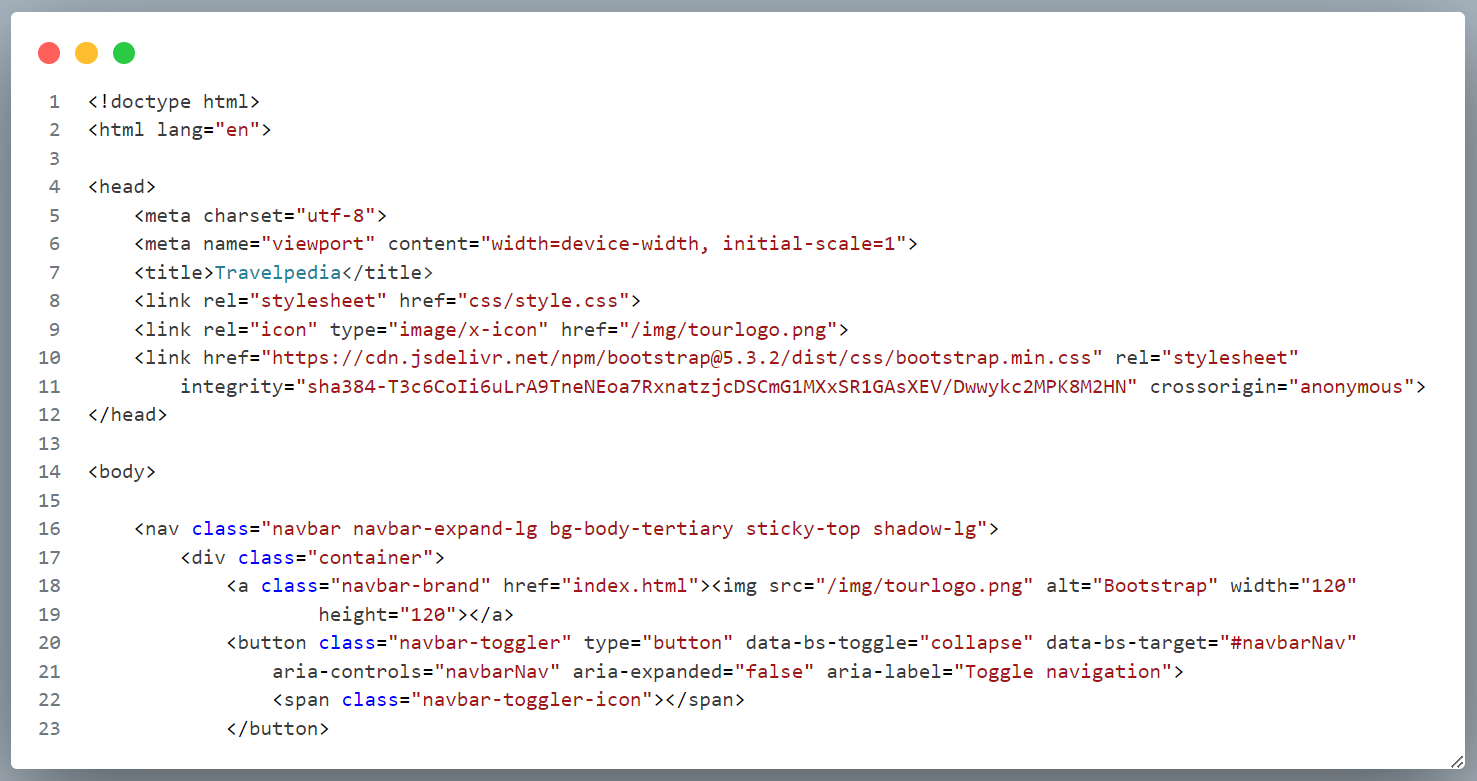
\includegraphics[width=16cm]{Gambar/bab2/html.png}
	\caption{Kode HTML}
	\label{fig:kode-html}
\end{figure}
\FloatBarrier

%%%%%%%%%%%%%%%%%%%%%%%%%%%%%%%%%%%%%%%%%%%%%%%%
\begin{figure}[!htbp]
	\centering
	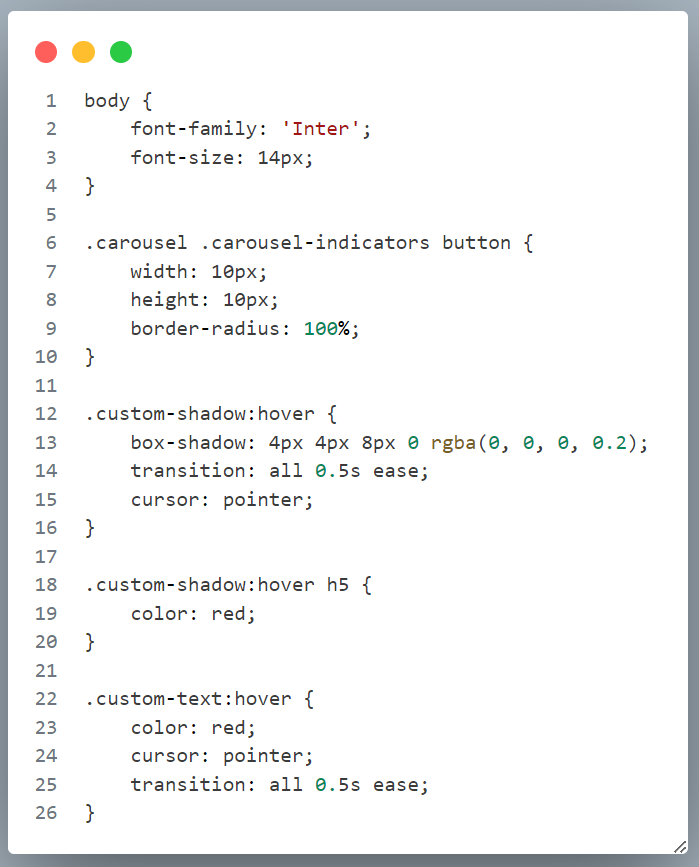
\includegraphics[width=7cm]{Gambar/bab2/css.png}
	\caption{Kode CSS}
	\label{fig:kode-css}
\end{figure}
\FloatBarrier

\subsubsection{JavaScript}
JavaScript adalah bahasa pemrograman dinamis yang terutama digunakan untuk membuat elemen interaktif pada halaman web. JavaScript memungkinkan pengembang untuk menambahkan berbagai fungsionalitas ke halaman web, termasuk validasi formulir, peta interaktif, grafik animasi, dan tata letak halaman web yang kompleks. Tidak seperti banyak bahasa pemrograman lainnya, JavaScript dieksekusi di browser pengguna (\textit{client-side})~\cite{basics2024unknown}. Dalam JavaScript, terdapat teknik bernama ajax yang berfungsi untuk membuat permintaan ke server untuk data tambahan tanpa perlu memuat ulang halaman web, yang menghasilkan pengalaman pengguna yang lebih baik~\cite{professional2023matt}. HTML DOM (\textit{Document Object Model}) merepresentasikan segala sesuatu di halaman HTML sebagai sebuah pohon Node, termasuk komentar HTML dan setiap spasi kosong. Semua elemen dalam DOM dapat diakses oleh JavaScript dan bisa diubah, dan setiap perubahan yang dilakukan oleh JavaScript akan langsung tercermin di halaman yang ditampilkan kepada pengguna~\cite{quick2023david}. Contoh kode JavaScript dapat dilihat pada \textbf{\ref{fig:kode-javascript}}.
%%%%%%%%%%%%%%%%%%%%%%%%%%%%%%%%%%%%%%%%%%%%%%%%
\begin{figure}[!htbp]
	\centering
	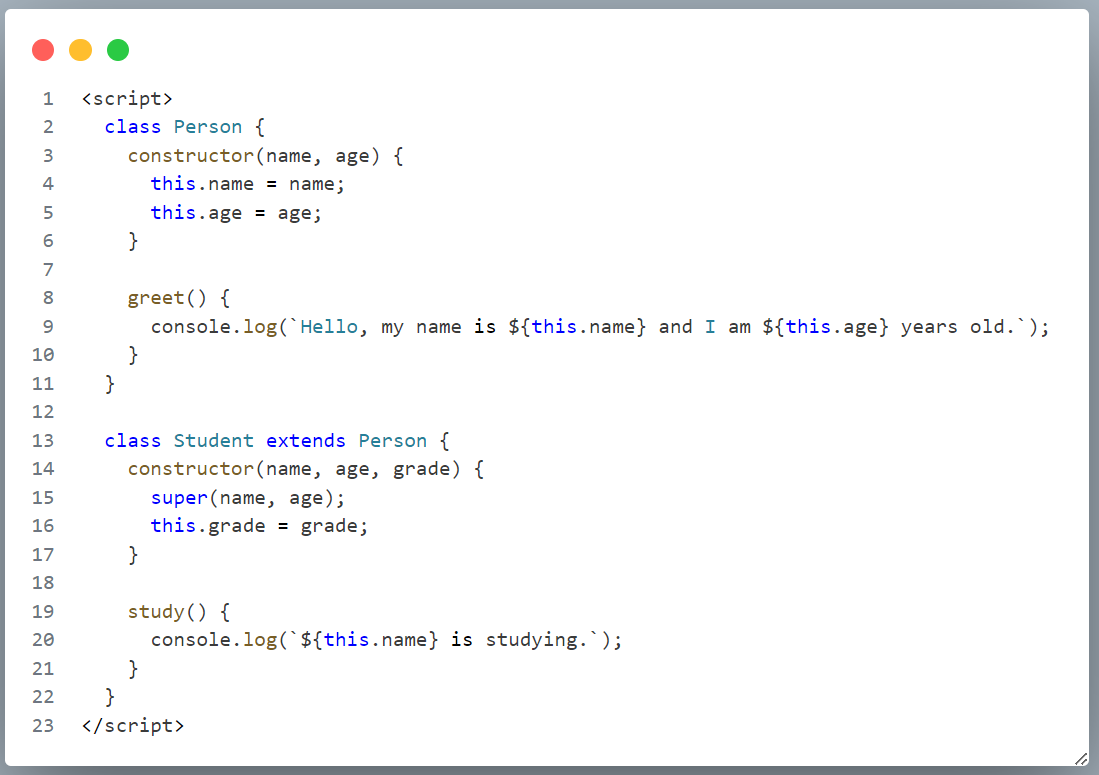
\includegraphics[width=14cm]{Gambar/bab2/javascript.png}
	\caption{Kode JavaScript}
	\label{fig:kode-javascript}
\end{figure}
\FloatBarrier

\subsubsection{PHP}
PHP adalah bahasa pemrograman yang berjalan di sisi server, berbeda dengan JavaScript yang merupakan bahasa pemrograman sisi klien~\cite{php2022tom}. PHP mendukung berbagai \textit{database} populer, seperti MySQL, PostgreSQL, Oracle, Sybase, Informix, dan \textit{Microsoft} SQL \textit{Server}, yang membuatnya fleksibel untuk berbagai kebutuhan pengembangan aplikasi web~\cite{php2022sufyan}. Contoh kode PHP dapat dilihat pada \textbf{\ref{fig:kode-php}}.
%%%%%%%%%%%%%%%%%%%%%%%%%%%%%%%%%%%%%%%%%%%%%%%%
\begin{figure}[!htbp]
	\centering
	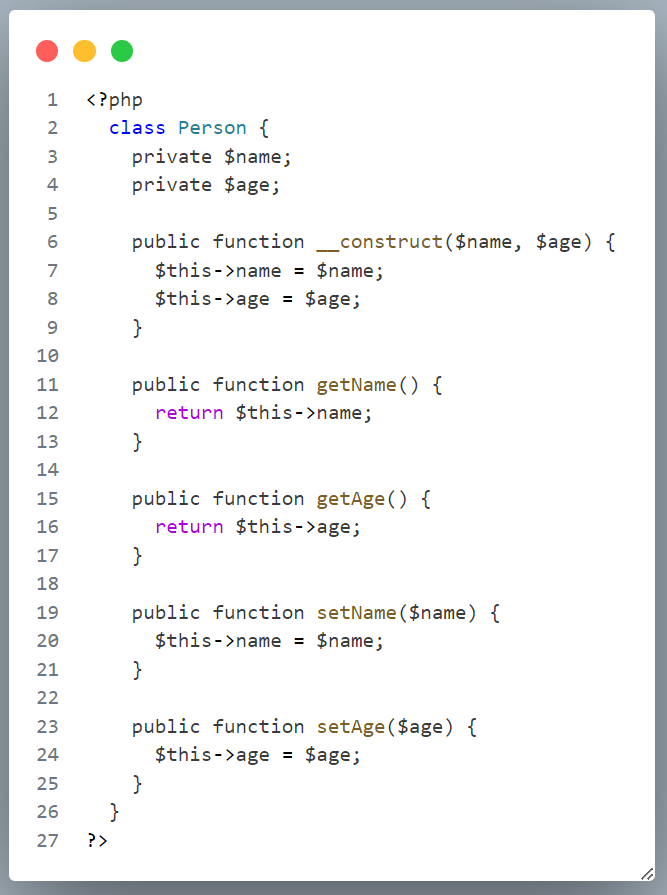
\includegraphics[width=8cm]{Gambar/bab2/php.png}
	\caption{Kode PHP}
	\label{fig:kode-php}
\end{figure}
\FloatBarrier

\subsubsection{JQuery}
jQuery bertujuan untuk menyederhanakan dan meningkatkan efisiensi penggunaan JavaScript dengan membuatnya lebih cepat, mudah, ringkas, dan menarik. \textit{Library} ini memungkinkan pengembang untuk membuat situs web yang lebih dinamis dan interaktif dengan memanfaatkan berbagai metode bawaan yang telah ditentukan. Dengan jQuery, banyak fungsi JavaScript yang biasa digunakan, yang biasanya memerlukan beberapa baris kode, dapat diakses dan dijalankan hanya dengan satu baris kode, sehingga mempercepat dan mempermudah proses pengembangan~\cite{masteringjquery2023sufyan}. Dokumentasi JQuery dapat diakses melalui \url{https://api.jquery.com/}. Contoh kode JQuery dapat dilihat pada \textbf{\ref{fig:kode-jquery}}.
%%%%%%%%%%%%%%%%%%%%%%%%%%%%%%%%%%%%%%%%%%%%%%%%
\begin{figure}[!htbp]
	\centering
	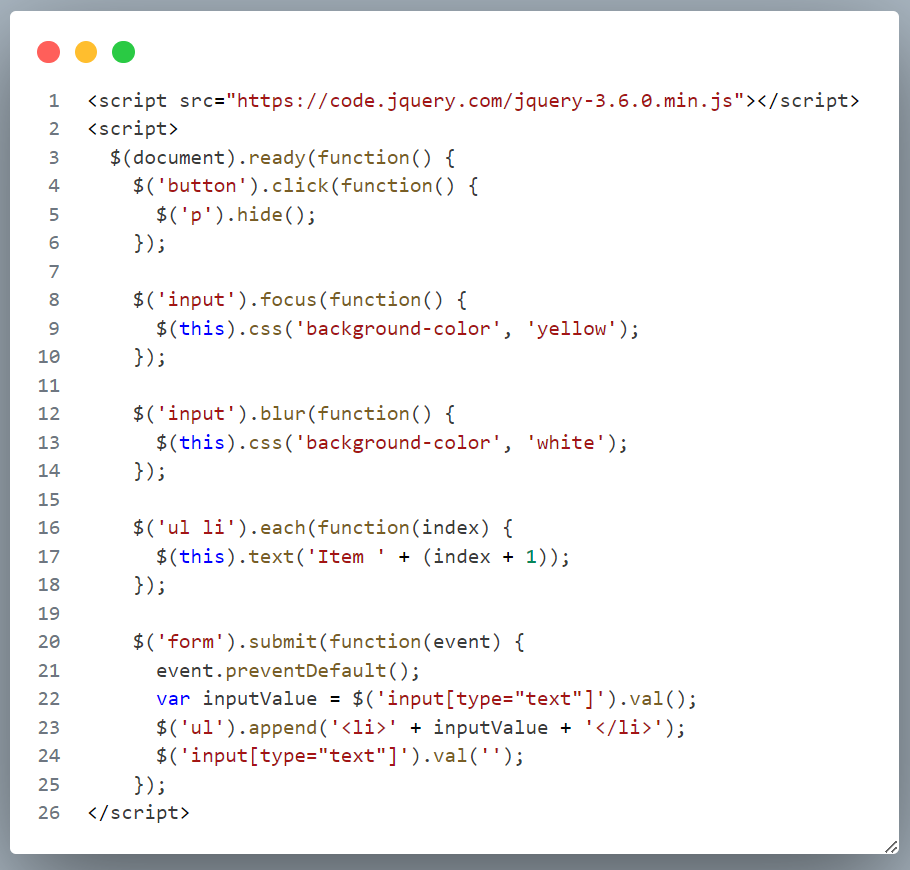
\includegraphics[width=10cm]{Gambar/bab2/jquery.png}
	\caption{Kode JQuery}
	\label{fig:kode-jquery}
\end{figure}
\FloatBarrier

\subsubsection{Laravel}
Laravel adalah \textit{framework} PHP yang gratis dan sumber terbuka yang menyediakan seperangkat alat dan sumber daya untuk membangun aplikasi web PHP modern. Laravel menyediakan sintaks yang elegan, fitur bawaan, dan berbagai paket serta ekstensi yang kompatibel. Saat pengembangan Laravel secara \textit{local}, membutuhkan XAMPP dan \textit{composer}. XAMPP adalah lingkungan pengembangan PHP yang paling populer. XAMPP adalah distribusi Apache yang gratis dan mudah diinstal yang mencakup MySQL, PHP, dan Perl. Composer adalah alat untuk mengelola ketergantungan dalam pengembangan PHP. Alat ini memudahkan mengelola \textit{libraries} yang dibutuhkan saat pengembangan proyek~\cite{practical2022daniel}. \textit{Framework} ini menyederhanakan berbagai tugas umum dalam pengembangan web, seperti interaksi dengan \textit{database}, autentikasi, antrian, pengiriman \textit{email}, dan \textit{caching}, berkat komponen-komponennya yang terintegrasi~\cite{laravel2023matt}. Dokumentasi Laravel dapat diakses melalui \url{https://laravel.com/docs/10.x/installation}. Kode \textit{command line} untuk instalasi \textit{framework} Laravel dengan composer dapat dilihat pada \textbf{\ref{fig:install-laravel}}. 
%%%%%%%%%%%%%%%%%%%%%%%%%%%%%%%%%%%%%%%%%%%%%%%%
\begin{figure}[!htbp]
	\centering
	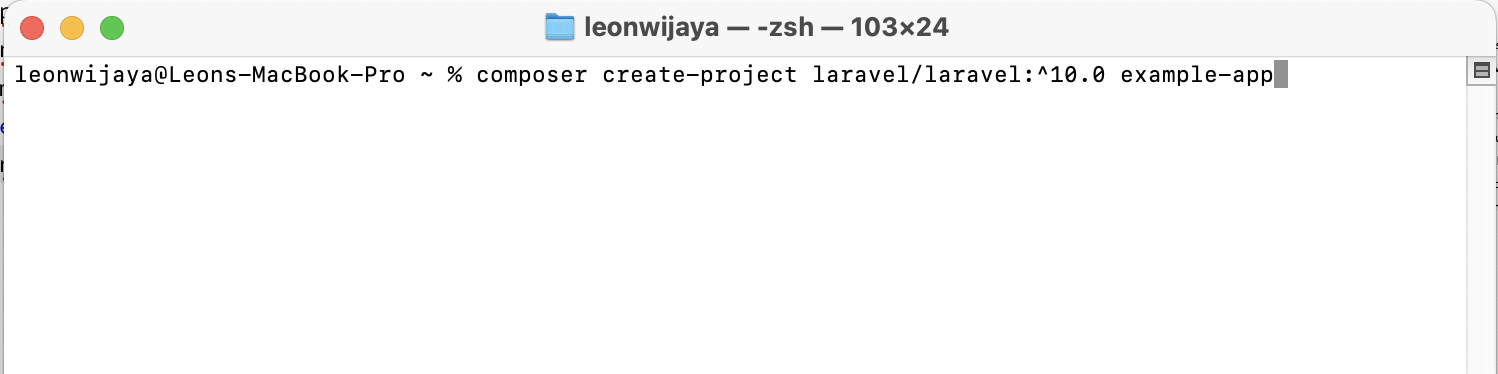
\includegraphics[width=8cm]{Gambar/bab2/install-laravel.png}
	\caption{Kode \textit{Command Line} Instalasi \textit{Framework} Laravel dengan Composer}
	\label{fig:install-laravel}
\end{figure}
\FloatBarrier

\subsubsection{TensorFlow}
TensorFlow adalah \textit{framework machine learning} yang memungkinkan pengembang untuk mengembangkan solusi \textit{machine learning} dengan cepat untuk berbagai kasus penggunaan khusus yang dapat memanfaatkan  \textit{machine learning}~\cite{thushan2022tensorflow}. TensorFlow dibuat di Google dan mendukung banyak aplikasi  \textit{machine learning} skala besar~\cite{hands2022aurelien}. TensorFlow memungkinkan pengembang untuk mendefinisikan dan melatih berbagai jenis model \textit{machine learning}, termasuk \textit{deep neural networks}, untuk berbagai tugas seperti \textit{classification}, \textit{regression}, \textit{clustering}, dan lain-lain~\cite{mastering2024hasan}. Pada aplikasi ini, model \textit{simple face detection (BlazeFace)} akan digunakan untuk mendeteksi wajah pada gambar selama pengambilan foto saat melakukan presensi. Dokumentasi TensorFlow dapat dilihat melalui \url{https://www.tensorflow.org/js/models}.

\subsubsection{Tailwind CSS}
Tailwind adalah sekumpulan kelas utilitas dasar yang dapat digunakan seperti blok penyusun untuk menciptakan berbagai desain yang kita inginkan. \textit{Framework} yang berfokus pada utilitas ini mencakup properti CSS yang paling penting, tetapi juga mudah diperluas dengan berbagai cara~\cite{tailwind2022ivaylo}. Tailwind CSS memiliki beberapa keunggulan, termasuk kemudahan dalam membuat prototipe, iterasi, dan kustomisasi tampilan, serta menyediakan \textit{modifier} untuk perilaku khusus. Selain itu, penggunaan Tailwind mengurangi penulisan CSS karena desain lebih banyak berasal dari komposisi \textit{utility}-nya~\cite{modern2022noel}. Dokumentasi Tailwind CSS dapat diakses melalui \url{https://tailwindcss.com/docs/installation}. Penulis menggunakan Tailwind CSS sebagai alat untuk mempermudah proses \textit{styling} pada tampilan aplikasi.


\subsubsection{Flowbite}
Flowbite merupakan \textit{library} komponen UI \textit{open source} yang dikembangakan dengan \textit{framework} Tailwind CSS yang berfokus pada pendekatan \textit{utility first}. \textit{Library} ini menyediakan berbagai komponen penting yang sering digunakan dalam pengembangan web, seperti tombol, \textit{dropdown}, \textit{navigation bar}, dan \textit{modal}~\cite{introduction2024flowbite}. Dokumentasi Flowbite dapat diakses melalui \url{https://flowbite.com/docs/getting-started/introduction/}. Penulis menggunakan Flowbite untuk mempercepat proses pembuata antarmuka pengguna (UI) karena terdapat komponen siap pakai.

\subsubsection{MySQL}
MySQL adalah sistem manajemen basis data relasional (RDBMS) sumber terbuka yang dikembangkan oleh perusahaan Swedia, MySQL AB. Perusahaan ini didirikan oleh David Axmark, Allan Larsson, dan Michael Widenius, dengan pengembangan awal MySQL dimulai oleh Widenius dan Axmark pada tahun 1994~\cite{masteringmysql2022sufyan}. MySQL banyak digunakan oleh beberapa organisasi dan pengembang karena beberapa alasan utama diantaranya yaitu bersifat open-source dan biasanya gratis, kinerja yang sangat cepat, mudah di-\textit{install} dan digunakan~\cite{mysql2023ben}.
